\begin{center}
\Huge
Polynomiel regression
\end{center}
\section*{Polynomiel regression}
\stepcounter{section}

Nøjagtigt som vi har set det med lineære, eksponentielle og potensfunktioner kan vi også lave
\textit{polynomiel regression}. Har vi et datasæt, vi antager kan beskrives af et polynomium af grad $n$, så kan vi lave polynomiel regression i Maple ved kommandoen
\begin{align*}
	&\texttt{restart} \\
	&\texttt{with(Gym):} \\
	&\texttt{PolyReg(data,n)} 
\end{align*}
hvor \texttt{data} er vores datasæt. 
\begin{exa}
	Vi får givet \href{https://github.com/ChristianJLex/TeachingNotes/raw/master/2023-2024/Data og lign/poly_example.xlsx}{\color{blue!60} dette datasæt} og forventer, at det kan beskrives af 
	et tredjegradspolynomium. Vi importerer det til Maple og laver polynomiel regression ved at 
	skrive
	\begin{align*}
		&\texttt{restart}\\
		&\texttt{with(Gym):}\\
		&\texttt{PolyReg(data,3)}
	\end{align*}
	Resultatet af dette kan ses af Figur \ref{fig:polyreg}.
	\begin{figure}[H]
		\centering
		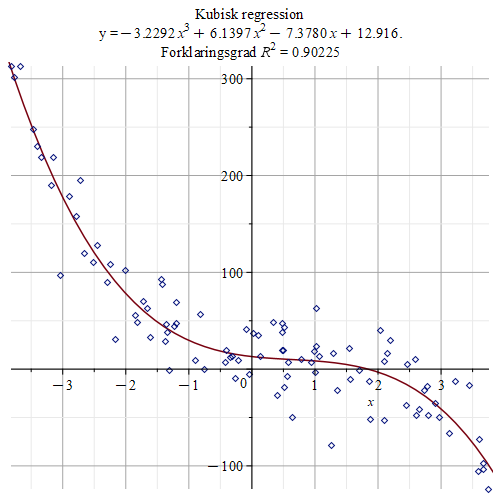
\includegraphics[width=0.7\textwidth]{Billeder/polyreg2}
		\caption{Polynomiel regression af 3. grad}
		\label{fig:polyreg}
	\end{figure}
	Hvis vi er interesserede i, hvor godt polynomiet beskriver datasættet, kan vi anvende 
	residualplottet. Dette får vi frem ved i Maple at skrive
	\begin{align*}
		\texttt{plotResidualer(data,[PolyReg,3])}
	\end{align*}
	Plottet kan ses af Figur \ref{fig:polyresidual}.
	\begin{figure}[H]
		\centering
		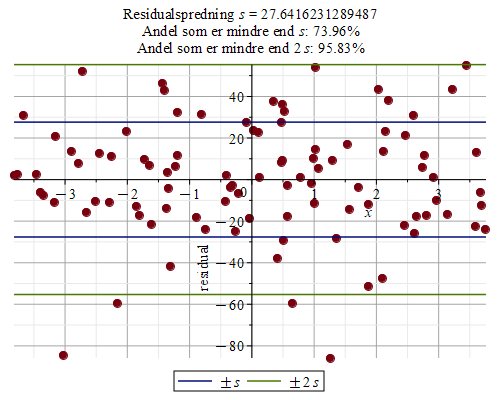
\includegraphics[width=0.7\textwidth]{Billeder/polyresidual}
		\caption{Residualplot for polynomiel regression}
		\label{fig:polyresidual}
	\end{figure}
	Af Figur \ref{fig:polyresidual} kan vi se, at residualerne ser tilfældigt spredte ud. 
	Derfor tror vi på, at modellen beskriver datasættet godt. 
\end{exa}
Det er vigtigt at bemærke, at vi altid skal vælge den polynomiumsmodel, der har lavest grad og som ser ud til at beskrive datasættet godt. Dette skal vi gøre, da vi i princippet kan beskrive datasættet vilkårligt godt med en høj nok polynomiel grad, men dette gør, at vi mister den underliggende sammenhæng mellem $x$- og $y$-værdierne. 

\subsection*{Opgave 1}
	Et datasæt er givet \href{https://github.com/ChristianJLex/TeachingNotes/raw/master/2023-2024/Data og lign/poly_opgave1.xlsx}{\color{blue!60} her}.
	\begin{enumerate}[label=\roman*)]
		\item Brug residualplots til at bestemme den mindste polynomielle grads regression, 
		der beskriver datasættet godt. 
		\item Lav polynomiel regression med den grad, du har bestemt i i) og bestem 
		forskriften for det polynomium, der beskriver datasættet.
		\item Brug forskriften til at bestemme $f(4)$.
		\item Brug Maple til at finde rødderne for $f$.
	\end{enumerate}
\subsection*{Opgave 2}
	Et datasæt er givet \href{https://github.com/ChristianJLex/TeachingNotes/raw/master/2023-2024/Data og lign/poly_opgave2.xlsx}{\color{blue!60} her}.
	\begin{enumerate}[label=\roman*)]
		\item Brug residualplots til at bestemme den mindste polynomielle grads regression, 
		der beskriver datasættet godt. 
		\item Lav polynomiel regression med den grad, du har bestemt i i) og bestem 
		forskriften for det polynomium $g$, der beskriver datasættet.
		\item Brug forskriften til at bestemme løsningen til ligningen $g(x)=12$
		\item Brug Maple til at finde rødderne for $g$.
	\end{enumerate}
	
\subsection*{Opgave 3}
	Et datasæt er givet \href{https://github.com/ChristianJLex/TeachingNotes/raw/master/2023-2024/Data og lign/poly_opgave3.xlsx}{\color{blue!60} her}.
	\begin{enumerate}[label=\roman*)]
		\item Brug residualplots til at bestemme den mindste polynomielle grads regression, 
		der beskriver datasættet godt. 
		\item Lav polynomiel regression med den grad, du har bestemt i i) og bestem 
		forskriften for det polynomium $h$, der beskriver datasættet.
		\item Brug Maple til at finde rødderne for $h$.
	\end{enumerate}

\subsection*{Opgave 4}
	Et datasæt er givet \href{https://github.com/ChristianJLex/TeachingNotes/raw/master/2023-2024/Data og lign/poly_opgave4.xlsx}{\color{blue!60} her}.
	\begin{enumerate}[label=\roman*)]
		\item Brug residualplots til at bestemme den mindste polynomielle grads regression, 
		der beskriver datasættet godt. 
		\item Lav polynomiel regression med den grad, du har bestemt i i) og bestem 
		forskriften for det polynomium $p$, der beskriver datasættet.
		\item Bestem skæringspunkterne mellem $p$ og $h$
	\end{enumerate}
	
\subsection*{Opgave 5}
	Et datasæt er givet \href{https://github.com/ChristianJLex/TeachingNotes/raw/master/2023-2024/Data og lign/poly_opgave5.xlsx}{\color{blue!60} her}.
	\begin{enumerate}[label=\roman*)]
		\item Brug residualplots til at bestemme den mindste polynomielle grads regression, 
		der beskriver datasættet godt. 
		\item Lav polynomiel regression med den grad, du har bestemt i i) og bestem 
		forskriften for det polynomium $q$, der beskriver datasættet.
		\item Tegn $q$ på intervallet $[-10,10]$. Har $q$ et maksimum eller minimum på dette interval?
	\end{enumerate}

\subsection*{Opgave 6}
	Et datasæt er givet \href{https://github.com/ChristianJLex/TeachingNotes/raw/master/2023-2024/Data og lign/poly_opgave6.xlsx}{\color{blue!60} her}.
	\begin{enumerate}[label=\roman*)]
		\item Brug residualplots til at bestemme den mindste polynomielle grads regression, 
		der beskriver datasættet godt. 
		\item Lav polynomiel regression med den grad, du har bestemt i i) og bestem 
		forskriften for det polynomium $r$, der beskriver datasættet.
		\item Løs ligningen $r(x) + p(x) = q(x)$.
	\end{enumerate}
